\documentclass[ignorenonframetext,aspectratio=169]{beamer}
\usetheme{metropolis}
\usepackage{fontspec}
\usepackage{hyperref}
\usepackage[czech]{babel}
\usepackage{multicol}
\usepackage{lipsum}
\usepackage{lua-widow-control}

\newtheorem{priklad}{Příklad}
\newtheorem{pozor}{Pozor}
\addtobeamertemplate{block begin}{\setlength\abovedisplayskip{0pt}}{}
\addtobeamertemplate{block end}{\vspace*{-1em}}{}
\newcommand\prepinac[1]{\texttt{-\/-#1}}


\newcommand\myfig[3][width=.9\textwidth]{%
  \figure\includegraphics[#1]{#2}%
  \caption{#3}%
\endfigure}

\author{Michal Hoftich}
\institute{Charles University, Faculty of Education, Library}
\title{LaTeX to Web publishing}

\begin{document}
\begin{frame}
\maketitle
\end{frame}

\begin{frame}
\tableofcontents
\end{frame}
% the slide input didn't work
% see https://tex.stackexchange.com/a/29355/2891
\mode<all>

\section{Úvod}

\begin{frame}
  \frametitle{Co je cílem?}
    Vytvořit z různých zdrojů (HTML, ePub) PDF vhodné pro několik výstupů:
    \begin{itemize}
      \item čtečky e-booků
      \item smartphony a tablety
      \item tisk
    \end{itemize}

  \end{frame}
  \begin{frame}
    \frametitle{Proč?}

    \begin{itemize}
      \item Komfortnější čtení
      \item Archivace
    \end{itemize}


\end{frame}

\section{Jak zkonvertujeme HTML do PDF pro čtečku?}

\begin{frame}
  \frametitle{Rmodepdf}

  Skript, který zkonvertuje webovou stránku nebo ePub soubor do PDF.

  \begin{itemize}
    \item extrahuje čistý text článků, bez reklam a navigačních elementů na stránkách
    \item měl by umožňovat konfiguraci pro jednotlivé weby nebo vydání e-booků (např. MK Praha)
    \item konfigurovatelný výstup
  \end{itemize}


    
  Rozpracovaný kód se nachází zde:

    \url{https://github.com/michal-h21/rmodepdf/}
  \end{frame}

\begin{frame}
  \frametitle{Reader mode pro skripty}
  Zobrazení pro čtečku je mód ve webových prohlížečích, který odstraní ovládací prvky ze stránky a zobrazí jen text článku.

  \bigskip

  \begin{tabular}{ll}
    Readability.js & \url{https://github.com/mozilla/readability}\\
    Python-readability & \url{https://github.com/buriy/python-readability}\\
    Rdrview: &\url{https://github.com/eafer/rdrview}\\
  \end{tabular}

\end{frame}

\begin{frame}
  \frametitle{Stránka s ovládacími prvky a reklamami}
  \begin{center}
    
\includegraphics[height=.9\textheight]{img/root-balast.png}
  \end{center}
\end{frame}

\begin{frame}
  \frametitle{Stránka v zobrazení čtečky}
  \begin{center}
    \includegraphics[height=.9\textheight]{img/root-čtečka.png}
  \end{center}
\end{frame}

\begin{frame}
  \frametitle{Jak načteme HTML a ePub soubory?}
  V Lua\TeX u máme několik nástrojů
  \begin{itemize}
    \item knihovna pro čtení ZIP souborů
    \item LuaXML obsahuje knihovnu Transform pro převod XML do jiných formátů, například \TeX u
      \begin{itemize}
        \item umožňuje pravidla pro specifické elementy vybrané pomocí CSS selektorů
      \end{itemize}
    \item podpora pro HTML v LuaXML je ve vývoji
  \end{itemize}
\end{frame}

\begin{frame}
  \frametitle{Co dále?}
  \begin{itemize}
  \item  zautomatizovat design výstupního dokumentu pro různé velikosti zobrazení
  \item  automaticky zamezit chybám v sazbě:
    \begin{itemize}
      \item vdovy a sirotci
      \item zalamování řádků s jednopísmennými předložkami, jednotkami nebo ak. tituly
      \item přetečené řádky při sazbě úzkých sloupců
    \end{itemize}
  \end{itemize}
\end{frame}

\section{Responzivní design v \LaTeX u}

\begin{frame}
   \frametitle{Co je responzivní design}
   \begin{itemize}
     \item flexibilní struktura - přizpůsobení velikosti prvků na stránce zobrazovacímu zařízení
     \item media queries - pravidla, která se aplikují na základě vlastností zobrazovacího zařízení (velikost displeje, druh displeje, atd.) 
   \end{itemize}

   Díky těmto vlastnostem může stejný kód stránky být dobře zobrazen jak na velkém monitoru, tak na mobilních zařízeních.
\end{frame}

\begin{frame}
  \frametitle{Balíček \texttt{responsive}}

  Balíček inspirovaný metodami responzivního designu pro webové stránky
  \begin{itemize}
  \item přizpůsobení velikosti fontu velikosti zobrazení
  \item typografická stupnice pro velikosti písma
  \item media queries
\end{itemize}
  \url{https://github.com/michal-h21/responsive-latex}
    % - změny počtu znaků na řádek
    % - okraje pomocí newgeometry
\end{frame}


\begin{frame}[fragile]
  \frametitle{Nastavení velikosti písma podle velikosti displeje}

  Velikost písma můžeme nastavit pomocí příkazu \verb|\setsizes{počet znaků na řádek}|.
  

\begin{columns}
  \begin{column}{0.5\textwidth}
\begin{verbatim}
\begin{minipage}{5cm}
\setsizes{25}

\lipsum[1]

\end{minipage}
\end{verbatim}
\end{column}
\begin{column}{0.5\textwidth}
\fbox{%
\begin{minipage}{5cm}
\ResponsiveSetup{lineratio=38}
\setsizes{25}

\normalsize


Lorem ipsum dolor sit amet,
consectetuer adipiscing elit.
Ut purus elit, vestibulum ut,
placerat ac, adipiscing vitae,
felis. 

\end{minipage}}
\end{column}
\end{columns}

\end{frame}

\begin{frame}[fragile]
  \frametitle{Rozdíl velikosti písma v závislosti na počtu znaků}
\begin{columns}
  \begin{column}{0.5\textwidth}
\begin{verbatim}
\setsizes{55}
\end{verbatim}
\fbox{%
\begin{minipage}{5cm}
\setsizes{55}

\lipsum[1]

\end{minipage}}
\end{column}
\begin{column}{0.5\textwidth}
\begin{verbatim}
\setsizes{25}
\end{verbatim}
\fbox{%
\begin{minipage}{5cm}
\ResponsiveSetup{lineratio=38}
\setsizes{25}

\normalsize


Lorem ipsum dolor sit amet,
consectetuer adipiscing elit.
Ut purus elit, vestibulum ut,
placerat ac, adipiscing vitae,
felis. 

\end{minipage}}
\end{column}
\end{columns}
\end{frame}

\begin{frame}[fragile]
  \frametitle{Konfigurace}
  Volby můžeme nastavovat při volání balíčku, nebo později pomocí příkazu \verb|\ResponsiveSetup|.

  Důležité volby:

  \begin{description}
    \item[noautomatic] -- nenastavovat velikost písma automaticky na začátku dokumentu
    \item[characters] -- počet znaků při automatickém nastavení velikosti písma
    \item[scale] --  typografická stupnice použitá pro velikosti řezů písma
    \item[lineratio] -- poměr využitý při výpočtu výšky řádku
  \end{description}

\end{frame}

\begin{frame}[fragile]
  \frametitle{Výška řádků}
  Výšku řádků můžeme ovlivnit pomocí volby \texttt{lineratio}. 
Čím vyšší má hodnotu, tím je vzdálenost mezi řádky menší.

\begin{columns}
  \begin{column}{0.5\textwidth}
\begin{verbatim}
\ResponsiveSetup{lineratio=38}
\end{verbatim}
\fbox{%
\begin{minipage}{5cm}
\ResponsiveSetup{lineratio=38}
\setsizes{55}

\lipsum[1]

\end{minipage}}
\end{column}
  \begin{column}{0.5\textwidth}
\begin{verbatim}
\ResponsiveSetup{lineratio=34}
\end{verbatim}
\fbox{%
\begin{minipage}{5cm}
\ResponsiveSetup{lineratio=34}
\setsizes{55}

\lipsum[1]

\end{minipage}}
\end{column}
\end{columns}

\end{frame}

\newcommand\printsize[1]{\csname #1\endcsname\par\noindent Sample\par}
\newcommand\showscale[2][.5\textwidth]{%
      % \setsizes[38]{25}
      \printsize{huge}
      \printsize{LARGE}
      \printsize{Large}
      \printsize{large}
      \hrule
      \printsize{normalsize}
      \hrule
      \printsize{small}
      \printsize{footnotesize}
}



\begin{frame}[fragile]
  \frametitle{Řezy písma}

  Velikosti jednotlivých řezů písma jsou vybírány na základě typografické stupnice

\begin{columns}
  \begin{column}{0.5\textwidth}
Defaultní stupnice (pentatonická)
\fbox{%
\begin{minipage}{5cm}
\setsizes{45}

\showscale{}

\end{minipage}}
\end{column}
  \begin{column}{0.5\textwidth}
\begin{verbatim}
\ResponsiveSetup{scale=golden}
\end{verbatim}
\fbox{%
\begin{minipage}{5cm}
\ResponsiveSetup{scale=golden}
\setsizes{45}

\showscale

\end{minipage}}
\end{column}
\end{columns}

\end{frame}

\begin{frame}[fragile]
  \frametitle{Jemnější nastavení stupnice}

  Můžeme také přímo nastavit poměr a počet kroků, za který se stupnice o tento poměr zvětší.

\begin{columns}
  \begin{column}{0.5\textwidth}
\begin{verbatim}
\ResponsiveSetup{ratio=2,
number=2,scale=none}
\end{verbatim}
\fbox{%
\begin{minipage}{5cm}
\ResponsiveSetup{ratio=2,
number=2,scale=none}
\setsizes{45}

\showscale{}

\end{minipage}}
\end{column}
  \begin{column}{0.5\textwidth}
\begin{verbatim}
\ResponsiveSetup{ratio=1.3,
number=2,scale=none}
\end{verbatim}
\fbox{%
\begin{minipage}{5cm}
\ResponsiveSetup{ratio=1.3,
number=2,scale=none}

\setsizes{45}

\showscale

\end{minipage}}
\end{column}
\end{columns}

\end{frame}

\begin{frame}[fragile]
\frametitle{Ukázka media query v CSS}
\begin{verbatim}
body {
  color: green;
}
@media screen and (max-width: 600px) {
    body {
      color: blue;
    }
}
\end{verbatim}
          
\end{frame}

\begin{frame}
  \frametitle{Ukázka stránky na velkém monitoru}
  \begin{center}
    
\includegraphics[height=.9\textheight]{img/pedf-web-big.png}
  \end{center}
\end{frame}

\begin{frame}
  \frametitle{Ukázka stránky na malém displeji}
  \begin{center}
    \includegraphics[height=.9\textheight]{img/pedf-web-small.png}
  \end{center}
\end{frame}

\begin{frame}[fragile]
  \frametitle{Media queries v \LaTeX u}
    Pomocí příkazu \verb|\MediaQuery| můžeme testovat různé vlastnosti:
  
    \begin{itemize}
  \item velikost fyzické stránky
  \item délku řádku
  \item orientaci stránky
\end{itemize}

Další testy jdou snadno přidat

\end{frame}

\begin{frame}[fragile]

  \frametitle{Příklad Media Query}

  Tento příklad zobrazí méně písmen pokud je šířka textu menší, než 4 cm.

  
\begin{verbatim}
\mediaquery{max-textwidth=4cm}
{\setsizes{45}}{\setsizes{60}}
\end{verbatim}
\begin{columns}
  \begin{column}{0.5\textwidth}
\fbox{%
\begin{minipage}{5cm}
\mediaquery{max-textwidth=4cm}
{\setsizes{45}}
{\setsizes{60}}

\lipsum[1]

\end{minipage}}
\end{column}
  \begin{column}{0.5\textwidth}
\fbox{%
\begin{minipage}{3.9cm}
\mediaquery{max-textwidth=4cm}
{\setsizes{45}}
{\setsizes{60}}

\lipsum[1]

\end{minipage}}
\end{column}
\end{columns}

\end{frame}


\section{Automatická sazba}

\begin{frame}
  \frametitle{Balíček texttt{lua-widow-control}}
  \begin{itemize}
    \item každý odstavec sází dvakrát -- jeden s normálními parametry, druhý o jeden řádek delší
    \item vliv na rychlost by měl být malý
    
    \item pokud se najde parchant, vymění předešlý odstavec za verzi s řádkem navíc
  \end{itemize}
\end{frame}

\begin{frame}
  \frametitle{Ukázka sirotka}
  \begin{center}
    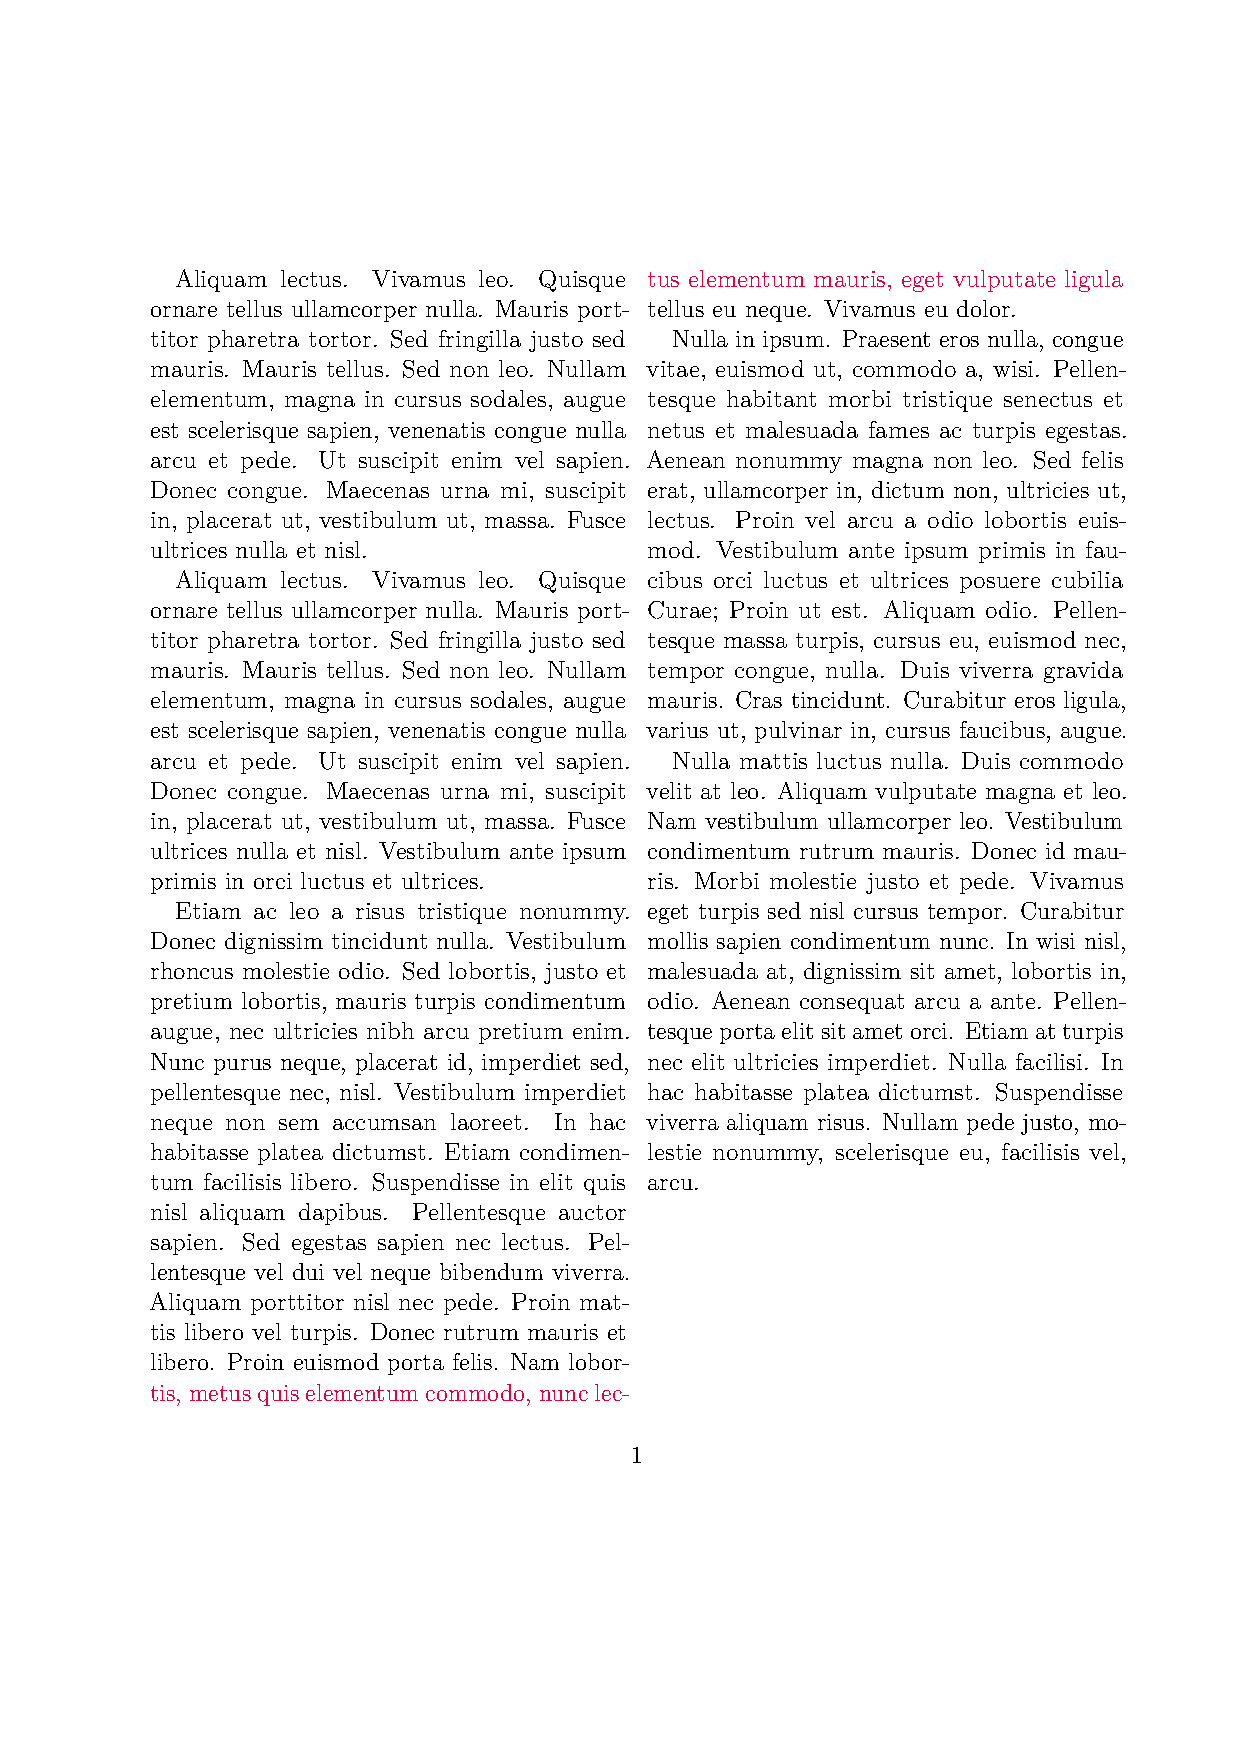
\includegraphics[height=\textheight,page=1]{examples/widow.pdf}
  \end{center}
\end{frame}

\begin{frame}
  \frametitle{Potlačený sirotek}
  \begin{center}
    \includegraphics[height=\textheight,page=2]{examples/widow.pdf}
  \end{center}
\end{frame}

\begin{frame}
  \frametitle{Porovnání různých metod k omezení parchantů}
  \begin{priklad}
  \begin{center}
  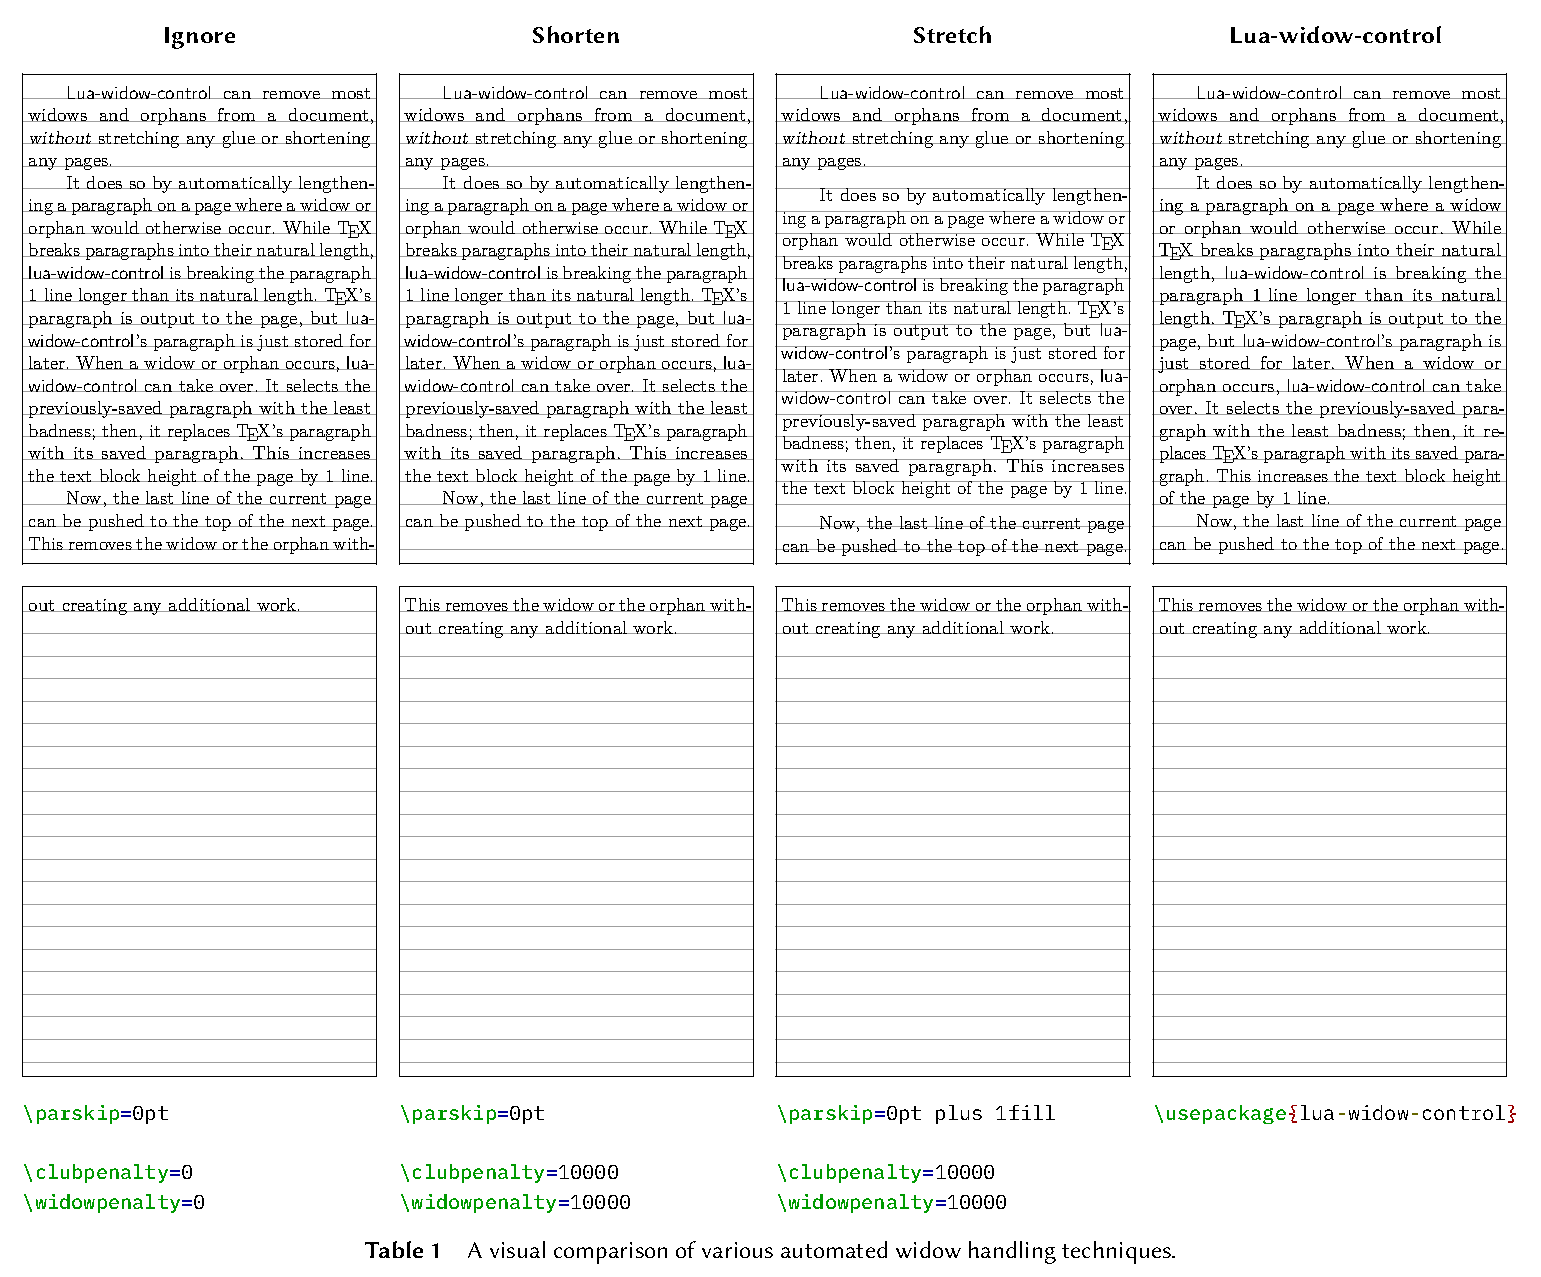
\includegraphics[height=.95\textheight]{img/lua-widow.pdf}
  \end{center}
\end{priklad}
  % \myfig[height=0.8\textheight]{img/lua-widow.pdf}{}
\end{frame}

\begin{frame}[fragile]
  \frametitle{Možnosti nastavení}
 \begin{verbatim}
 \lwcsetup{...}
 \end{verbatim}
 \begin{description}
   \item[default] -- nepřidává žádné vertikální mezery, ale může vést k příliš vzdušným odstavcům
   \item[strict] -- využívá primárně vertikální mezery a nevytváří špatné odstavce,  
     \begin{itemize}
       \item ale odstraní jen třetinu parchantů
        \item funguje špatně hlavně pro dokumenty, které obsahují jen text, beletrii apod.
      \end{itemize}
    \item[balanced] -- kombinuje obě metody, odstraní 90\% parchantů
  \end{description}
\end{frame}

\begin{frame}[fragile]
  \frametitle{Omezení}
    \begin{itemize}
      \item \verb|\clubpenalty| a \verb|\widowpenalty| nemají žádný efekt, naopak mohou způsobit vedlejší účinky
      \item  podpora pro více sloupcovou sazbu je omezená, balíček Multicol nefunguje
  \end{itemize}
\end{frame}
 

\begin{frame}[fragile]
  \frametitle{Balíček \texttt{luavlna}}
  \begin{itemize}
    \item Zamezuje rozdělení řádků:
      \begin{itemize}
        \item za jednoslovnými předložkami
        \item u iniciál
        \item u akademických titulů
        \item mezi čísly a jednotkami
      \end{itemize}
  \end{itemize}
\end{frame}

\begin{frame}
  \frametitle{Ukázka užití Luavlny}
  \begin{minipage}{3in}

    \preventsingledebugon

    Text s krátkými souhláskami a samohláskami i dalšími jevy
    z nabídky možností (v textu možnými).

    Co třeba í znaky š diakritikou?

    Různé možnosti [v závorkách \textless i jiných znacích

    Podpora iniciál a titulů: M. J. Hegel, Ing. Běháková, Ph.D., Ž. Zíbrt,
    Ch. Borner.

    Podpora jednotek: 100,5 MN\cdot{}s, 100.5 kJ, 200 µA, $-1$ dag.

    Uvnitř matematiky by mělo být zpracování vypnuté: $k \in \mathbb N$.

    \preventsingledebugoff
  \end{minipage}
\end{frame}

\begin{frame}
    \frametitle{Zalamování spojovníků}
    \begin{center}
    \begin{minipage}{2in}
      Sedlec-Prčice, modro-zelený, překladatel-tlumočník, kuchař-číšník, propan-butan, Otýlie Sklenářová-Malá, František Jílek-Oberpfalcer.
    \end{minipage}
  \end{center}
\end{frame}

\begin{frame}
  \frametitle{Volby balíčku}
  Pomocí voleb můžeme zakázat některé vlastnosti
  \begin{description}
    \item [noprocess] – nespouštět zpracování dokumentu automaticky
    \item [noinitials] – iniciály
    \item [nounits] – SI jednotky
    \item [nopredegrees] – tituly před jménem
    \item [nosufdegrees] – tituly za jménem
  \end{description}
\end{frame}

\begin{frame}[fragile]
  \frametitle{Užitečné příkazy}
  \begin{itemize}
    \item \verb|\singlechars{jazyk}{písmena}| -- seznam písmen, u kterých se potlačuje zalamování řádků

    \item \verb|\enablesplithyphens{jazyk}| -- nastaví podporu zalamování spojovníků pro daný jazyk
    \item \verb|\preventsinglelang{jazyk}| -- nastaví pravidla pro daný jazyk pro celý dokument
  \end{itemize}
\end{frame}

\begin{frame}[fragile]
  \frametitle{Podporované jazyky}
  Vestavěná podpora je pouze pro češtinu a slovenštinu:

\begin{verbatim}
\singlechars{czech}{AIiVvOoUuSsZzKk}
\singlechars{slovak}{AIiVvOoUuSsZzKk}
\end{verbatim}

Je třeba jazyk vybrat pomocí balíčků Babel nebo Polyglossia

\begin{verbatim}
A příklad česky.
\selectlanguage{english}
A something.
\end{verbatim}

    \preventsingledebugon

A příklad česky.
\selectlanguage{english}
A something.

    \preventsingledebugoff

    \selectlanguage{czech}

\end{frame}

\newcommand\testbox[1]{%
  \parbox{150pt}{%
    \parindent=15pt%
    \tolerance=1%
    \pretolerance=1%
    #1
  }%
}

\newcommand\printtest[1]{%
  \linebreakerdisable%
  \noindent\testbox{%
    #1
    \par\medskip\noindent\hfill\textbf{Bez Linebreakeru}\hfill\null
  }%
  \linebreakerenable%
  \hfill%
  \testbox{%
    #1
    \par\medskip\noindent\hfill\textbf{S Linebreakerem}\hfill\null
  }%
}


\begin{frame}
  \frametitle{Balíček \texttt{linebreaker}}
  \begin{itemize}
    \item brání výskytu přetečených řádků
    \item ovlivňuje pouze sazbu  odstavců, kde se takový řádek vyskytl
  \end{itemize}
\end{frame}
  
\begin{frame}
  \frametitle{Příklad}
  \printtest{
    The example document given below creates two pages by using Lua code alone. You
will learn how to access TeX's boxes and counters from the Lua side, shipout a
page into the PDF file, create horizontal and vertical boxes (hbox and vbox),
create new nodes and manipulate the nodes links structure. 
%The example covers the following node types: rule, whatsit, vlist, hlist and action.
  }

\end{frame}
 
\begin{frame}[fragile]
  \frametitle{Nastavení}
  Linebreaker můžeme konfigurovat pomocí příkazu \verb|\linebreakersetup|:
  \begin{description}
    \item[maxcycles] -- počet pokusů o přesázení odstavce
    \item[maxemergencystretch] -- maximální hodnota \verb|\emergencystretch|
    \item[maxtolerance]  -- maximální hodnota \verb|tolerance|
  \end{description}
\begin{verbatim}
\linebreakersetup{
maxtolerance = 90,
maxemergencystretch = 1em,
maxcycles = 4
}
\end{verbatim}

\end{frame}

\section{Závěr}

\begin{frame}[standout]
  Děkuji za pozornost!

  \url{michal.h21@gmail.com}

  \url{www.kodymirus.cz}

\end{frame}

\mode*
% % - problems with the hook insertion
%   - separation of presentation and content
% - issues with the generated code
%   - misuse of math commands for text 
% - sub/superscripts - https://tex.stackexchange.com/q/482081/2891
% - fonts - htf fonts, Fontspec


% \begin{frame}
%   \frametitle{Contents}
%   \tableofcontents
% \end{frame}



\begin{frame}
  \frametitle{Popular \TeX\ to HTML convertors}
  \begin{itemize}
    \item Pandoc
    \item LaTeXML
    \item LaTeX2HTML
    \item Lwarp
  \end{itemize}
\end{frame}

% \section{tex4ht conversion system}


\begin{frame}
  \frametitle{tex4ht overview}
  \begin{itemize}
    \item \url{https://www.tug.org/tex4ht/}
    \item created in the mid nineties
    \item original author Eitan Gurari (1947--2009)
    \item current team Michal Hoftich and Karl Berry 
    \item updates goes directly to \TeX\ Live
  \end{itemize}
\end{frame}

\begin{frame}
  \frametitle{Basic features}
  \begin{itemize}
    \item it uses \TeX\ for the compilation of the document \\(all formats in theory, mainly \LaTeX\ in practice)
    \item it can convert parts of the document to images
    \item it supports multiple output formats
  \end{itemize}

\end{frame}



% \begin{frame}
%   \frametitle{Three phase compilation}
%   \begin{itemize}
%     \item the document is compiled by \TeX\ with \texttt{tex4ht.sty} package autoloaded
%     \item processing of the \texttt{DVI} file by the \texttt{tex4ht} command
%     \item processing of the \texttt{.lg} file by the \texttt{t4ht} command
% \end{itemize}
% \end{frame}

\begin{frame}
  \frametitle{Overview of the compilation}
  \ifdefined\HCode
      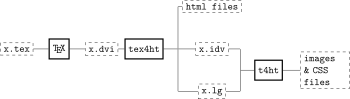
\includegraphics[width=600px]{img/tex4ht_process}
  \else
      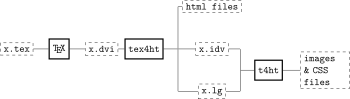
\includegraphics[width=\textwidth]{img/tex4ht_process}
  \fi
\end{frame}

\begin{frame}
  \frametitle{Compilation by \TeX\ with the \texttt{tex4ht.sty} package auto-loaded}
  \begin{itemize}
    \item loading configuration \texttt{.4ht} files for the supported packages
    \item patching commands with hooks 
    \item hooks configuration according to the output format
  \end{itemize}
\end{frame}

\begin{frame}
  \frametitle{DVI processing using the \texttt{tex4ht} command}
  \begin{itemize}
    \item   generation of the output files
    \item   font handling 
      \begin{itemize}
        \item based on the \texttt{.htf} files, they contain mappings between the font characters and Unicode 
        \item information about the font style
        \item character encoding conversion
        % \item basic text formatting
      \end{itemize}
    \item prepare \texttt{.lg} and \texttt{.idv} files

      % \begin{itemize} 
        % \item  poměrně komplikovaný proces, potřebujeme
          % doplňkové soubory pro fonty obsahující unicode entity nebo ASCII
          % znaky pro jednotlivé znaky písma
  % \end{itemize}
    % \item   zachovává základní styly písem, podporuje jakákoli makra měnící vzhled písma
    % \item   příprava .lg souboru
    % \item   zápis .idv souboru obsahující stránky pro konverzi na obrázky
  \end{itemize}
\end{frame}

\begin{frame}
  \frametitle{.lg file processing using the \texttt{t4ht} command}
  \begin{itemize}
    \item   CSS file
    \item   picture generation
    \item   external commands calling
    (\texttt{xslt}, \texttt{tidy}, \texttt{xmllint}, \texttt{xtpipes})
  \end{itemize}
\end{frame}

% \section{tex4ht configuration}
\begin{frame}
  \frametitle{How does \texttt{tex4ht.sty} work?}
  \begin{itemize}
    \item \texttt{tex4ht.sty} package is called before the document is lodaded by \TeX
    \item it modifies the document processing
    \item it detects all used packages and loads configuration \texttt{.4ht} files at the \texttt{\string\begin\{document\}}\\
    the configurable hooks are inserted into redefined commands
    \item another \texttt{.4ht} file with tags is included after the package configurations.\\ 
      It contains all configurations for the current output format
    % \item the tags are inserted into configurable hooks created in the previous step 
      
    % \item po zpracování preamble a nahrání všech balíčků se spouští .4ht soubory s vkládáním háčků pro dané balíčky, pokud existují
    \begin{pozor}<2>
      The commands used in the document preamble are not patched by \texttt{tex4ht} by default
    \end{pozor}
\end{itemize}
\end{frame}

\begin{frame}
  \frametitle{When is it necessary to insert the configurable hooks?}
  \begin{itemize}
\item when we want to keep the logical structure of the document
      (sectioning, tables, lists, etc.)
    \item in the case of a clash between existing \texttt{tex4ht} commands and commands provided by a package
  \end{itemize}
\end{frame}

\begin{frame}
  \frametitle{How are hooks configured}
  \begin{itemize}
    \item hooks are configured using the \texttt{\textbackslash Configure} command
    \item either in the output format file (html4.4ht, html5.4ht, ooffice.4ht)
    \item or in the private configuration file
    \item the output format can define options that are passed to the \texttt{tex4ht.sty} package
    % \item soubory výstupního formátu mohou definovat volby, které ovlivňují konfiguraci háčků
    % \item po vložení háčků se nahrají jejich konfigurace v závislosti na výstupním formátu
    % \item další konfigurace je možné vložit do .cfg souboru, který se načítá pomocí volby \texttt{-c} příkazu \texttt{make4ht}

\end{itemize}
\end{frame}

\begin{frame}[fragile]
  \frametitle{\texttt{tex4ht.sty} package options}
    they are used by the output format for a conditional configuration

  \begin{itemize}
    \item they can be passed on the command line
    \item or in a private configuration file 
  \end{itemize}
  \begin{priklad}
\begin{verbatim}
$ make4ht filename.tex "mathml,mathjax"
\end{verbatim}
\end{priklad}
\end{frame}

\begin{frame}
  \frametitle{Some available options}
\begin{itemize}
  \item fn-in
  \item pic-m, pic-align
  \item svg
  \item info
  \item mathml
  \item mathjax
\end{itemize}
\end{frame}


\begin{frame}[fragile]
  \frametitle{Private configuration file}
  \begin{itemize}
    \item Basic structure
      \begin{verbatim}
% \RequirePackage is possible to use here
\Preamble{xhtml, options}
\Configure{foo}{}{}
\Css{body{...}}
...
\begin{document}
...
\EndPreamble
      \end{verbatim}
  \end{itemize}
\end{frame}



\begin{frame}[fragile]
  \frametitle{Some available commands}
  \begin{itemize} 
  \item \verb|\Configure|, \verb|\ConfigureEnv|, \verb|\ConfigureList|
  \item \verb|\HCode|, \verb|\Css|, \verb|\Hnewline|
  \item \verb|\EndP|, \verb|\IgnorePar|
  \item \verb|\Picture+|, \verb|\Picture*|
  \item \verb|\NoFonts|, \verb|\EndNoFonts|
\end{itemize}
\end{frame}

\begin{frame}[fragile]
  \frametitle{Example for the \texttt{\string\Configure} command}
  \begin{priklad}
\begin{verbatim}
\Configure{textit}
  {\HCode{<em>}\NoFonts}
  {\EndNoFonts\HCode{</em>}}
\end{verbatim}
  \end{priklad}
\end{frame}


\begin{frame}[fragile]
  \frametitle{Issues with paragraphs}
  \begin{priklad}
\begin{verbatim}
\ConfigureEnv{rightaligned}
    {\HCode{<section class="right">}}
    {\HCode{</section>}}{}{}
\end{verbatim}
\end{priklad}
The generated HTML code is invalid
\begin{priklad}
\begin{verbatim}
<p class="indent" ><section class="right">
\end{verbatim}
\end{priklad}
\end{frame}

\begin{frame}[fragile]
  \frametitle{A correct solution}
  \begin{priklad}
\begin{verbatim}
\ConfigureEnv{rightaligned}
    {\ifvmode\IgnorePar\fi\EndP%
     \HCode{<section class="right">}\par}
    {\ifvmode\IgnorePar\fi\EndP%
     \HCode{</section>}}{}{}
\end{verbatim}
  \end{priklad}

  Result

  \begin{verbatim}
<section class="right">
<!--l. 9--><p class="indent" >
  \end{verbatim}
\end{frame}

\begin{frame}[fragile]
  \frametitle{Pictures}
  \begin{priklad}
\begin{verbatim}
\ConfigureEnv{topicture}
  {\Picture*{}}
  {\EndPicture}
  {}{}
\end{verbatim}
\end{priklad}
\end{frame}

\begin{frame}[fragile]
  \frametitle{Complete configuration file}
    \small
    \begin{verbatim}
\Preamble{xhtml}
\Configure{textit}
   {\HCode{<em>}\NoFonts}
   {\EndNoFonts\HCode{</em>}}
\ConfigureEnv{rightaligned}
   {\ifvmode\IgnorePar\fi\EndP
    \HCode{<section class="right">}\par}
   {\ifvmode\IgnorePar\fi\EndP
    \HCode{</section>}}{}{}
\ConfigureEnv{topicture}
   {\Picture*{}}{\EndPicture}{}{}
\Css{.right{text-align:right;display:block;}}
\begin{document}
\EndPreamble
  \end{verbatim}
\end{frame}

% \begin{frame}[fragile]
% \frametitle{Example with options}
% \begin{verbatim}
% \Preamble{xhtml,mathml,2,sec-filename,fn-in,fonts}
% % external stylesheet
% \Configure{AddCss}{style.css}
% \begin{document}
% \EndPreamble
% \end{verbatim}
% \end{frame}

% \begin{frame}[fragile]
%   \frametitle{Konfigurace mini obsahu na jednotlivých stránkách}
%   \small
%   \begin{verbatim}
% \Configure{crosslinks+}{%
%   \bgroup
%   \Configure{tableofcontents}
%   {\IgnorePar\EndP
%   \HCode{<nav class="TOC">}\IgnorePar}
%   {\HCode{\Hnewline}}
%   {\IgnorePar\HCode{</nav>\Hnewline}\ShowPar}{}{}%
%   \TableOfContents[chapter,section,subsection]
%   \egroup
%   \ifvmode\IgnorePar\fi\EndP%
%   \HCode{<article class="main-content">\Hnewline
%   <nav class="crosslinks-top">}}
%   {\HCode{</nav>\Hnewline}}
% {\ifvmode\IgnorePar\fi\EndP%
%   \HCode{<nav class="crosslinks-bottom">}}
%   {\HCode{</nav>}}{}{}
%   \end{verbatim}
% \end{frame}

% \begin{frame}[fragile]
%   \frametitle{Další nastavení}
%   \begin{verbatim}
% % uzavřít <article>, který byl otevřen v 
% % \Configure{crosslinks+}
% \Configure{@/BODY}
% {\ifvmode\IgnorePar\fi\EndP\HCode{</article>}}

% % Ukázat odkazy pouze na předešlou, 
% % hlavní a násladující stránku
% \Configure{crosslinks*}{prev}{up}{next}{}
% \begin{document}
% \EndPreamble
% \end{verbatim}
% \end{frame}

% \section{Přidání podpory pro nové balíčky}

\begin{frame}
  \frametitle{How to add support for a new package?}
  \begin{itemize}
    \item create file named \texttt{package name + .4ht}, redefine commands and insert configurable hooks here
    \item configure the hooks in the output format \texttt{.4ht} file
  \end{itemize}
\end{frame}


\begin{frame}[fragile]
  \frametitle{Sample package  }
\texttt{custom.sty:}
  \begin{verbatim}
\ProvidesPackage{custom}
\newcommand\custom[1]{\bgroup\itshape#1\egroup}
\endinput
  \end{verbatim}
% \end{frame}
\medskip
\texttt{custom.4ht:}
% \begin{frame}[fragile]
  % \frametitle{Insert hooks in the \texttt{custom.4ht} file}
  \begin{verbatim}
\NewConfigure{custom}{2}
\pend:defI\custom{\a:custom}
\append:defI\custom{\b:custom}
\Hinput{custom}
  \end{verbatim}
\end{frame}

\begin{frame}[fragile]
  \frametitle{Configure the hooks for the \texttt{HTML} output}
  \begin{verbatim}
\Configure{custom}
    {\HCode{<span class="custom">}\NoFonts}
    {\EndNoFonts\HCode{</span>}}
\end{verbatim}
\end{frame}


%\begin{frame}[fragile]
%  \frametitle{Vlastní výstupní formát \texttt{myoutput.4ht}}
%  \begin{verbatim}
%\exit:ifnot{custom} 
%\ConfigureHinput{custom} 
%\Configure{custom}
%{\HCode{<span class="custom">}\NoFonts}
%{\EndNoFonts\HCode{</span>}}
%\endinput\empty\empty\empty\empty\empty\empty 
%%%%%%%%%%%%%%%%%%%%%%%%%%%%%%%%%%%%%%%%%%%%%%%
%\endinput 
%  \end{verbatim}
%\end{frame}

%\begin{frame}[fragile]
%  \frametitle{Definice vlastního formátu \texttt{tex4ht.usr}}
%  \begin{verbatim}
%\Configure{myoutput}{% 
%   \Hinclude[*]{html4.4ht}%
%   \Hinclude[*]{unicode.4ht}%
%   \Hinclude[*]{html5.4ht}%
%   \Hinclude[*]{myoutput.4ht}% 
%} 
%  \end{verbatim}
%\end{frame}

%\begin{frame}[fragile]
%  \frametitle{Kompilace vlastního formátu}
%  \begin{verbatim}
%make4ht -um draft sample.tex myoutput
%  \end{verbatim}
%\end{frame}
\begin{frame}

  \frametitle{Scripts}
  \begin{itemize}
    \item high number of compilation scripts
    \item the basic script was \texttt{htlatex} 
    \item the difference between the scripts is just in used options
    \item superseded by \texttt{make4ht}
\end{itemize}
\end{frame}

\begin{frame}[fragile]
  \frametitle{Traditional compilation scripts}
  \begin{itemize}
    \item bash scripts for UNIX, batch scripts for Windows
    % \item parametry pro každý jednotlivý krok se předávají kompilačnímu skriptu v závorkách
    \item parameters can be passed for each command used in the tex4ht compilation
  \end{itemize}
\end{frame}

% \section{The \texttt{make4ht} build system}
\begin{frame}
  \frametitle{\texttt{htlatex} issues}
  \begin{itemize}
    \item difficult way of passing the arguments to \texttt{htlatex}
    \item fixed compilation sequence
      \begin{itemize}
        \item \TeX\ is always executed three times
        \item it is not possible to use Bib\TeX\ or similar tools
      \end{itemize}
    \item it is hard to modify the image conversion process
    \item copying of files to an output directory doesn't work correctly
    \item post-processing of the generated files
  \end{itemize}
\end{frame}

\begin{frame}
  \frametitle{tex4ebook}
  \begin{itemize}
    \item support for e-books
    \item written in Lua
    \item simplified interface, use of command line switches
    \item Lua build file support
      \begin{itemize}
        \item call external commands
        \item picture generation process simplified
        \item post-processing of the generated files
      \end{itemize}
    \item extensions
    \item it keeps the correct directory structure with the \texttt{--output-dir} option
  \end{itemize}
\end{frame}

\begin{frame}
  \frametitle{make4ht}
  \begin{itemize}
    \item evolved from \texttt{tex4ebook}
    \item supports all \texttt{tex4ht} output formats
  \end{itemize}

\end{frame}


\begin{frame}[fragile]
  \frametitle{\texttt{htlatex} versus \texttt{make4ht}}
      % \begin{priklad}
        \small
\begin{verbatim}
$ htlatex filename.tex \ 
"tex4ht.sty options" "tex4ht options" \
"t4ht options" "TeX options"
\end{verbatim}

versus

\begin{verbatim}
$ make4ht [make4ht switches] filename.tex \ 
"tex4ht.sty options" "tex4ht options" \
"t4ht options" "TeX options"
\end{verbatim}
      % \end{priklad}
\end{frame}

\begin{frame}[fragile]
  \frametitle{How to get the UTF-8 encoded document?}
% \begin{priklad}
        \small 
\begin{verbatim}
$ htlatex filename.tex "xhtml,charset=utf-8" 
" -cmozhtf -utf8"
\end{verbatim}
     % \end{priklad}
% \end{frame}
% \begin{frame}[fragile]
  % \frametitle{Výstup v kódování  UTF8}
     versus
      % \begin{priklad}
\begin{verbatim}
$ make4ht -u filename.tex
\end{verbatim}
% \end{priklad}

\end{frame}


\begin{frame}[fragile]
  \frametitle{\texttt{make4ht} switches}
\begin{description}
  \item[\prepinac{utf8 (-u)}] 
  \item[\prepinac{mode (-m)}] 
  \item[\prepinac{lua (-l)}] 
  \item[\prepinac{config (-c)}] 
  \item[\prepinac{build-file (-e)}] 
  \item[\prepinac{output-dir (-d)}] 
  \item[\prepinac{shell-escape (-s)}] 
  \item[\prepinac{xetex (-x)}] 
  \item[\prepinac{format (-f)}] 
\end{description}

\end{frame}

\begin{frame}
  \frametitle{Supported formats}
  \texttt{make4ht}
  \begin{itemize}
    \item html5
    \item xhtml
    \item odt
    \item TEI
    \item DocBook
    \item etc.
  \end{itemize}
  \texttt{tex4ebook}
  \begin{itemize}
    \item ePub
    \item ePub3
    \item mobi
  \end{itemize}
\end{frame}

\begin{frame}[fragile]
  \frametitle{Extensions}
  \begin{priklad}
\begin{verbatim}
$ make4ht -f html5+tidy simple-example.tex
\end{verbatim}
\end{priklad}
\end{frame}

\begin{frame}
  \frametitle{Available extensions}
\begin{description}
  \item latexmk\_build
  \item tidy
  \item dvisvgm\_hashes
  \item common\_filters and common\_domfilters
  \item mathjaxnode -- example \url{https://www.kodymirus.cz/samples/mathjaxnode/maths.html}
  \item staticsite
\end{description}
\end{frame}

% \begin{frame}[fragile]
%   \frametitle{Konfigurační soubor .make4ht}
%   \begin{priklad}
% \begin{verbatim}
% filter_settings "staticsite" {
%   site_root = "output" 
% }

% Make:enable_extension("common_domfilters")
% if mode=="publish" then
%   Make:enable_extension("staticsite")
%   Make:htlatex()
% end
% \end{verbatim}
% \end{priklad}

% \end{frame}

% \begin{frame}[fragile]

%   \frametitle{Kompilace}

%   \begin{priklad}
% \begin{verbatim}
% make4ht -um publish simple-example.tex
% \end{verbatim}
% \end{priklad}
% \end{frame}

% \begin{frame}[fragile]
%   \frametitle{Výsledný HTML soubor}
%   \begin{priklad}
% \begin{verbatim}
% ---
% time: 1544811015
% date: '2018-12-14 18:10:47'
% title: 'sample'
% styles:
% - '2018-12-14-simple-example.css'
% meta:
% - charset: 'utf-8'
% ---
% <p>Sample document</p>
% \end{verbatim}
% \end{priklad}
% \end{frame}

% \subsection{Build file sample}
\begin{frame}[fragile]

\frametitle{Problematic document}
\begin{priklad}
\begin{verbatim}
\documentclass{article}
\begin{document}
Test {\itshape háčků}
\end{document}
\end{verbatim}
\end{priklad}
\end{frame}

\begin{frame}[fragile]
  \frametitle{Part of the generated HTML file}
\begin{priklad}
\begin{verbatim}
<!--l. 4--><p class="noindent" >Test <span 
class="rm-lmri-10">h</span><span 
class="rm-lmri-10">á</span><span 
class="rm-lmri-10">čk</span><span 
class="rm-lmri-10">ů</span> </p> 
\end{verbatim}
\end{priklad}

\end{frame}


\begin{frame}[fragile]
  \frametitle{Sample build file}
  \begin{priklad}
\begin{verbatim}
local domfilter = require("make4ht-domfilter")
local function domsample(dom)
  for _, par in ipairs(dom:query_selector("p")) do
    par:set_attribute("class", "mypar")
  end
  return dom
end
local process = domfilter({
  "joincharacters", 
  domsample})
Make:match("html$", process)
\end{verbatim}
  \end{priklad}
\end{frame}

\begin{frame}[fragile]
  \frametitle{Upravený HTML kód}
  \begin{priklad}
\begin{verbatim}
<!-- l. 3 --><p class='mypar'>
Test <span class='rm-lmri-10'>háčků</span> 
</p> 
\end{verbatim}
  \end{priklad}
\end{frame}

\begin{frame}[fragile]
  \frametitle{Build file with external commands}
  \texttt{sample.mk4}
  % \begin{priklad}
\begin{verbatim}
Make:add("biber","biber ${input}")
Make:htlatex {}
Make:biber {}
Make:htlatex {}
Make:image("png$",                                                          
  "dvipng -bg Transparent -T tight -o ${output}"..
  "-pp ${page} ${source}")
\end{verbatim}
  % \end{priklad}
\medskip

\begin{verbatim}
$ make4ht -e sample.mk4 filename.tex
\end{verbatim}
\end{frame}



\begin{frame}
\frametitle{That's all}
\begin{block}{}
Thanks for your attention.

Questions? 
\end{block}
\end{frame}


\end{document}
